% Use a one-sided article template
\documentclass[oneside]{article}
% Decrease the margins a little
\usepackage{fullpage}

% Set up for including graphics
% We'll use png or pdf graphics
\usepackage[pdftex]{graphicx}
\DeclareGraphicsExtensions{.png,.pdf}

% Hyperref adds hyperlinks to the document automatically
% It's not much use yet, but it will be
\usepackage{hyperref}

% For including code into the document
\usepackage{verbatim}

% Tweak the default fonts a little
\renewcommand\rmdefault{bch}
\usepackage[small]{caption}
\usepackage[small]{titlesec}
\linespread{1.07} 

\title{Homework 1}
\author{Hadley Wickham}
\date{\today}

\raggedbottom

\begin{document}
\maketitle 

This sample document introduces you to some of the features of latex.  Like the introduction to R, you'll start of just by copying this template and modifying it to meet your needs.  As the semester goes on you'll learn more about exactly what you're doing and explore more of the many advanced features of latex.  

As you can see from this text, basic text in latex is very easy.  You just type normal paragraphs (with a blank line between them).  Unlike word, you don't need to worry about the appearance of the text - latex takes care of laying it out for you.  For special formatting, use {\bf bold} or {\it italics} or \verb|some_R_code()|.  You'll notice that in latex most special formatting commands use the backslash and brackets - \verb|\|, \verb|{| and \verb|}|.  

Quotes are a little tricky: use `` '' (\verb|Shift + ~| on the left), or ` ', but never "".  

In the remainder of this document you'll see how to:

\begin{itemize}
  \item Make lists (like this one).
  \item Create headings and subheadings.
  \item Include images.
  \item Include code.
\end{itemize}

\section{Headings}

In latex headings are created with the {\tt section} command (like above).  Subheadings are created with {\tt subsection} and sub-subsections with {\tt subsubsection}.  Headings are automatically numbered and will be included in a table of contents if you have one.  (If you want to include a table of contents, just insert \verb|\tableofcontents| where you want it.)

\section{Images}

To include images you use the \verb|\includegraphics| command.  It looks like this:

\begin{verbatim}
\includegraphics{table-depth}
\includegraphics[width = 2in]{table-depth}
\includegraphics[width = 0.5\linewidth]{table-depth}
\end{verbatim} 

Notice that you don't include the file extension - latex will figure it out (this makes it easier to change the file format without having to go back and change the document).

If you want to include two images on the same line that take up exactly half the page each, you'll need a \% (a comment) after the first:

\includegraphics[width = 0.5\linewidth]{table-depth}%
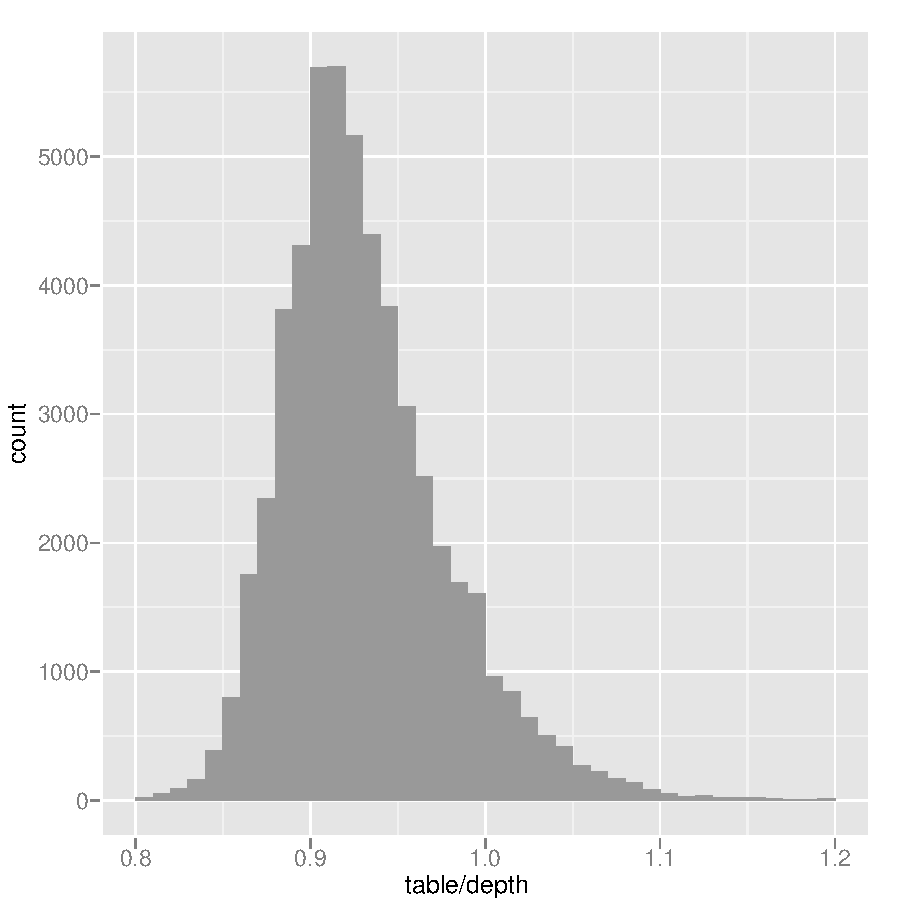
\includegraphics[width = 0.5\linewidth]{table-depth-ratio}

If you have a plot with thousands of points (like the above scatterplot), use png output, otherwise use pdf. I'll leave it up to you to figure out how to get three or four plots on a line.

\section{Figures and cross references}

Instead of inserting images directly into the text, you can insert them into a figure.  Figures will move around to where there is enough space and can have captions and labels.  A label allows you to add a reference to the figure like so:  Figure \ref{fig:two} is on page \pageref{fig:two}.  Figures should always be placed after where they are referenced in the text.

Getting figures to appear exactly where you want them in latex is a black art.  For homeworks, don't worry about it too much.  For many homeworks you will probably just want to place the images directly in the text, so it won't be a problem.

\begin{figure}[htbp]
  \includegraphics[width = 0.5\linewidth]{table-depth} %
  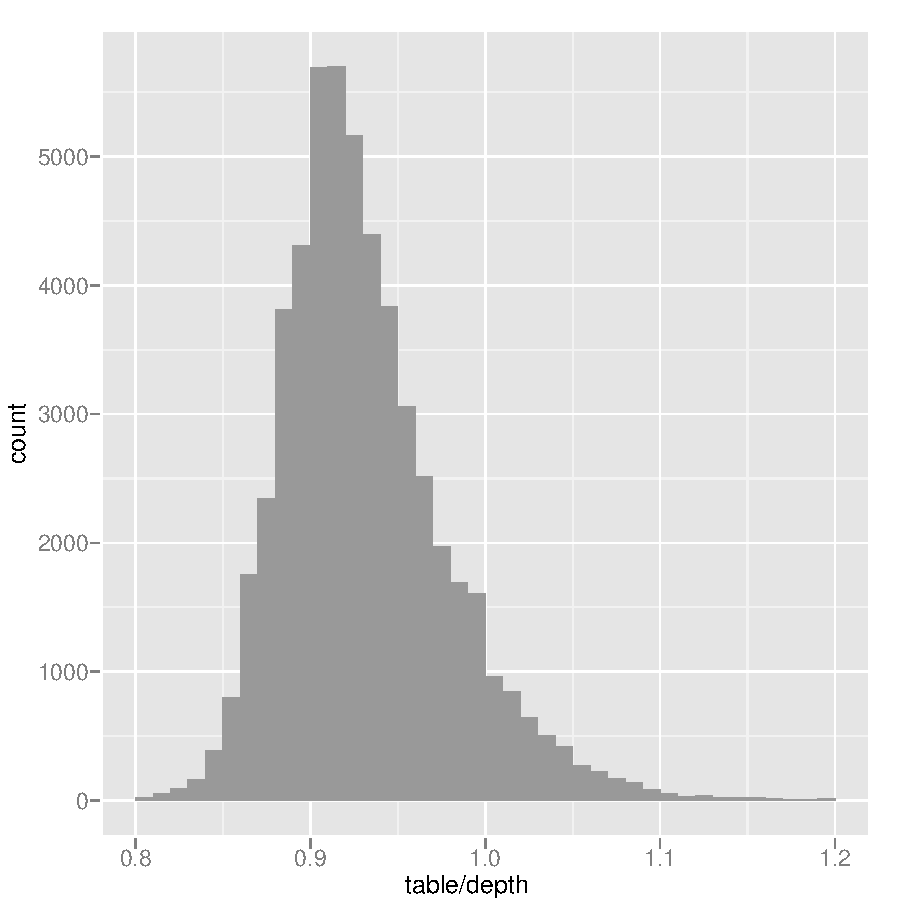
\includegraphics[width = 0.5\linewidth]{table-depth-ratio}
  \caption{(Left) A scatterplot of table vs. depth.  Note the vertical striations caused by the low resolution of the table variable. (Right) A histogram showing the ratio between table and depth, with bin width 0.01.  The distribution appears to be somewhat skew-right, centred around 0.9.}
  \label{fig:two}
\end{figure}

\begin{figure}[htbp]
  % If the figures don't fill up the whole line, include \centering
  % to centre them on the page.
  
  \centering
  \includegraphics[width = 2in]{table-depth}
  \caption{This is a bad caption because does not describe the figure, and it is not self-contained.}
  \label{fig:one}
\end{figure}

\newpage
\appendix
\section{Code}

Your homework should always include an appendix containing the code that you used.  (Look at the latex commands to see how I created the appendix) The \verb|verbatiminput| command takes a path to the file name that you want to include.  Verbatim means just include the raw text, without interpreting any special latex codes (look for the other verbatim commands that I've used in this document.)

The code should be self-contained so that running (e.g.) \verb|source("code.r")| from R doesn't produce any errors and produces all the graphics necessary for the homework.

\verbatiminput{code.r}

\end{document}
